\lab{Applications}{Plotting With Matplotlib and Mayavi}{Plotting}
\objective{Introduce some of the basic plotting functions available in
Matplotlib and Mayavi}
\label{lab:Matplotlib_and_Mayavi}

\section*{matplotlib}
Matplotlib is one of Python's many plotting libraries. Its high quality
and user interface explains why matplotlib serves as our primary
plotting library for 2D graphs in this text. It has an active
development community and was designed to resemble MATLAB.

Matplotlib has many different plotting functions and we strongly
encourage you to visit \url{http://matplotlib.org} for more
information.

\subsection*{Simple Plots} 
The basic line plotting function in matplotlib is \li{plot}. It takes a
set of data points and plots the line that is formed between those points. 
These plots are pieced together using a state machine environment, meaning that 
we can run several different functions and they will all display or modify the 
plot we are creating. 

To get started, import pyplot from matplotlib.
\begin{lstlisting} 
from matplotlib import pyplot as plt
\end{lstlisting}

To plot and show our function we typically use something like:
\begin{lstlisting} 
plt.plot(x,y) 
plt.show() 
\end{lstlisting}

The user provides the x and y coordinates of these points. It is important that the 
coordinates provided are the same dimension for \li{plot} to work. 

We can generate a basic plot of $e^x$ using the following lines of code:
\begin{lstlisting}
x = np.linspace(-2, 3, 501) # linspace(start, stop, num=50)  
y = np.exp(x)
plt.plot(x, y)
plt.show() 
\end{lstlisting}

Notice that \li{linspace} is extremely useful in plotting since it produces evenly spaced values between a given interval. The default number of these evenly spaced values is 50, but was adjusted in the previous code to be 501. It returns these values in an \li{ndarray}. 

This should display a plot similar to the one shown in Figure
\ref{fig:exp_plot}.

\begin{figure}
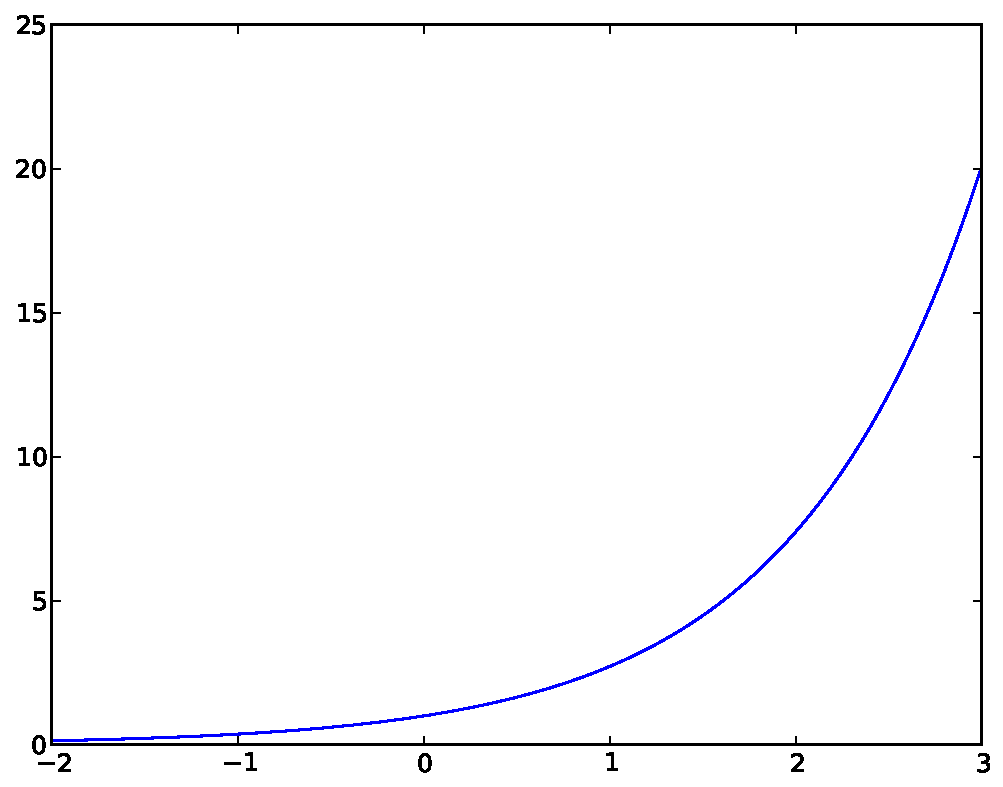
\includegraphics[width=\textwidth]{exp_plot.pdf}
\caption{A simple plot of $e^x$.} 
\label{fig:exp_plot} 
\end{figure}

\subsection*{Multiple Plots}
We can use the state based interface to display multiple plots at once. 
The following code will plot lines with random values at integers from 1 to 10. 
Note that \li{random.rand} creates an array of the given shape and propagates it with random samples from a uniform distribution over [0,1). Obviously, the given dimensions should be positive and if no argument is given, a single float is returned. 

\begin{lstlisting}
x = np.linspace(1, 10, 10) 
y = np.random.rand(10, 10) # Produces random values in a 10x10 size array.
plt.plot(x, y[0], x, y[1], x, y[2], x, y[3], x, y[4], x, y[5], x, y[6], x, y[7], x, y[8], x, y[9])
plt.show() 
\end{lstlisting}

We just used the plot function to plot several different lines at once. Alternatively, we can plot each \li{(x, y[i])} pair separately and overlay the plots to produce the same result. 
\begin{lstlisting}
x = np.linspace(1, 10, 10) 
y = np.random.rand(10, 10) 
plt.plot(x, y[0]) 
plt.plot(x, y[1]) 
plt.plot(x, y[2])
plt.plot(x, y[3]) 
plt.plot(x, y[4]) 
plt.plot(x, y[5]) 
plt.plot(x, y[6])
plt.plot(x, y[7]) 
plt.plot(x, y[8]) 
plt.plot(x, y[9]) 
plt.show()
\end{lstlisting}
A more efficient way to create this plot would be with a loop.
\begin{lstlisting}
x = np.linspace(1, 10, 10) 
y = np.random.rand(10, 10) 
for n in y: 
    plt.plot(x, n) 
plt.show()
\end{lstlisting}
A plot that was generated by this code will be similar to the one shown
in Figure \ref{fig:statemachine}.

\begin{figure}
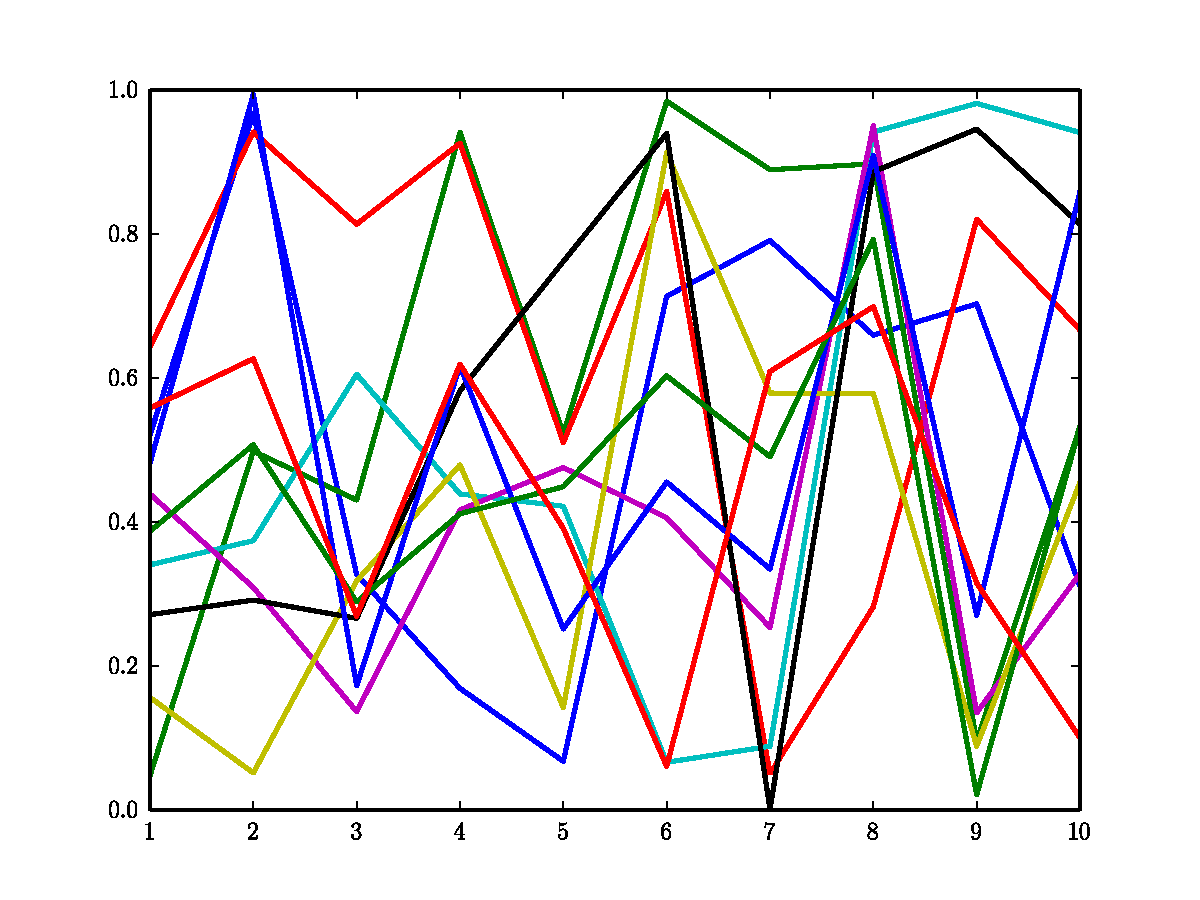
\includegraphics[width=\textwidth]{statemachine.pdf}
\caption{A plot of $10$ lines with randomly generated $y$ values.}
\label{fig:statemachine} 
\end{figure}

Note that a suitable domain and range for your plot is automatically chosen 
unless specified otherwise. 

\begin{problem} Plot the function $\sin(x)$ from $0$ to $2\pi$ with a red dashed line. Then plot the function $\cos(x)$ on the same domain with a blue dotted line using a single call to the plot function. More information on how to do this can be found in Appendix \ref{mpltables}. 
\end{problem}


\begin{comment}
There are also many functions that we may use to set different values in
the plotting environment. A few examples are shown in Table
\ref{mpl:useful_functions}.

\begin{table}
\begin{center} 
\begin{tabular}{|l|p{6cm}|p{4cm}|}

    \hline

    Function & Description & Usage\\

    \hline

    \li{annotate} & adds a commentary at a given point on the plot &
    annotate('text',(x,y))\\

    \li{arrow} & draws an arrow from a given point on the plot &
    arrow(x,y,dx,dy)\\

    \li{axhline} & draws a horizontal line at y from xmin to xmax &
    axhline(y=0, xmin=0, xmax=1)\\

    \li{axvline} & draws a vertical line at x from ymin to ymax &
    axvline(x=0, ymin=0, ymax=1)\\

    \li{axhspan} & draws a rectangle from xmin to xmax and ymin to ymax,
    if no xmin and xmax are given it goes across the plot &
    axhspan(ymin, ymax, xmin=0, xmax=1)\\

    \li{axvspan} & draws a rectangle from ymin to ymax and xmin to xmax,
    if no ymin and ymax are given it goes across the entire plot &
    axvspan(xmin, xmax, ymin=0, ymin=1)\\

    \li{figlegend} & place a legend in the plot & figlegend(handles,
    labels, loc)\\

    \li{grid} & add gridlines & grid()\\

    \li{text} & add text at a given position on the plot &
    text(x,y,'text')\\

    \li{title} & add a title to the plot & title('text')\\

    \li{xlim} & set the x limits, returns current limits if no arguments
    are given & xlim(xmin,xmax)\\

    \li{ylim} & set the y limits, returns current limits if no arguments
    are given & ylim(ymin,ymax)\\

    \li{xticks} & set the location of the tick marks on the x axis,
    returns current locations if no arguments are given & xticks(x)\\

    \li{yticks} & set the location of the tick marks on the y axis,
    returns current locations if no arguments are given & yticks(y)\\

    \li{xlabel} & add a label to the x axis & xlabel('text')\\

    \li{ylabel} & add a label to the y axis & ylabel('text')\\

    \hline

    \end{tabular} 
    \end{center} 
    \caption{Some Functions to Set Plotting Options} 
    \label{mpl:useful_functions} 
    \end{table}

	\end{comment}
	
\begin{problem} 
Plot the curve $1/(x-1)$ from $-2$ to $6$ with a 
magenta dashed line. Force the plot to only show $y$ values that are between $-6$ and $6$. Make your line width 5. Once again, more information on how to do this can be found in Appendix \ref{mpltables}. 
By default, \texttt{plot} will try to make the graph connected. Correct this so that the graph appears to be discontinuous at $x=1$, as it should be, by modifying the input values. 

Your plot should look like the figure below.

\begin{figure}[H]
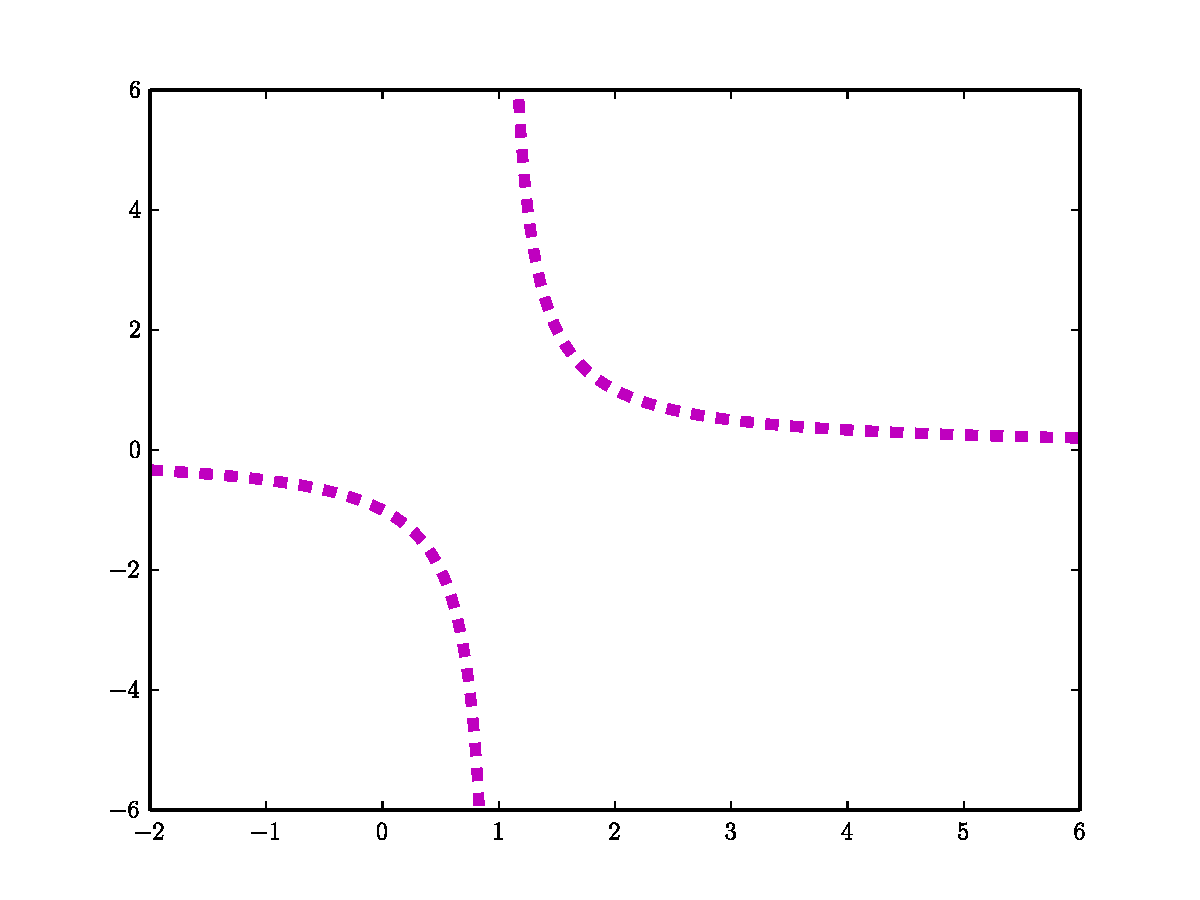
\includegraphics[width=\textwidth]{soln2.pdf}
\label{fig:problem2} 
\end{figure}
\end{problem}

\begin{problem} Plot the curve $\sin(x)\frac{1}{x+1}$ from $0$ to $10$.
Use blue shading under the curve when it is positive and red when it is
negative (Hint: you may want to use the \li{fill_between} command).
Make the line dotted. Label the x-axis ``x-axis'', the y-axis ``y-axis'',
and the plot ``My Plot''. Enable the gridlines.

Also include a scatter plot of half of the value of the function at each
of it's maxima and minima in the range. Have it display the points as
blue triangles. Make sure the x limits of the plot are still 0 and 10.

Your plot should look like the figure below.

\begin{figure}[H]
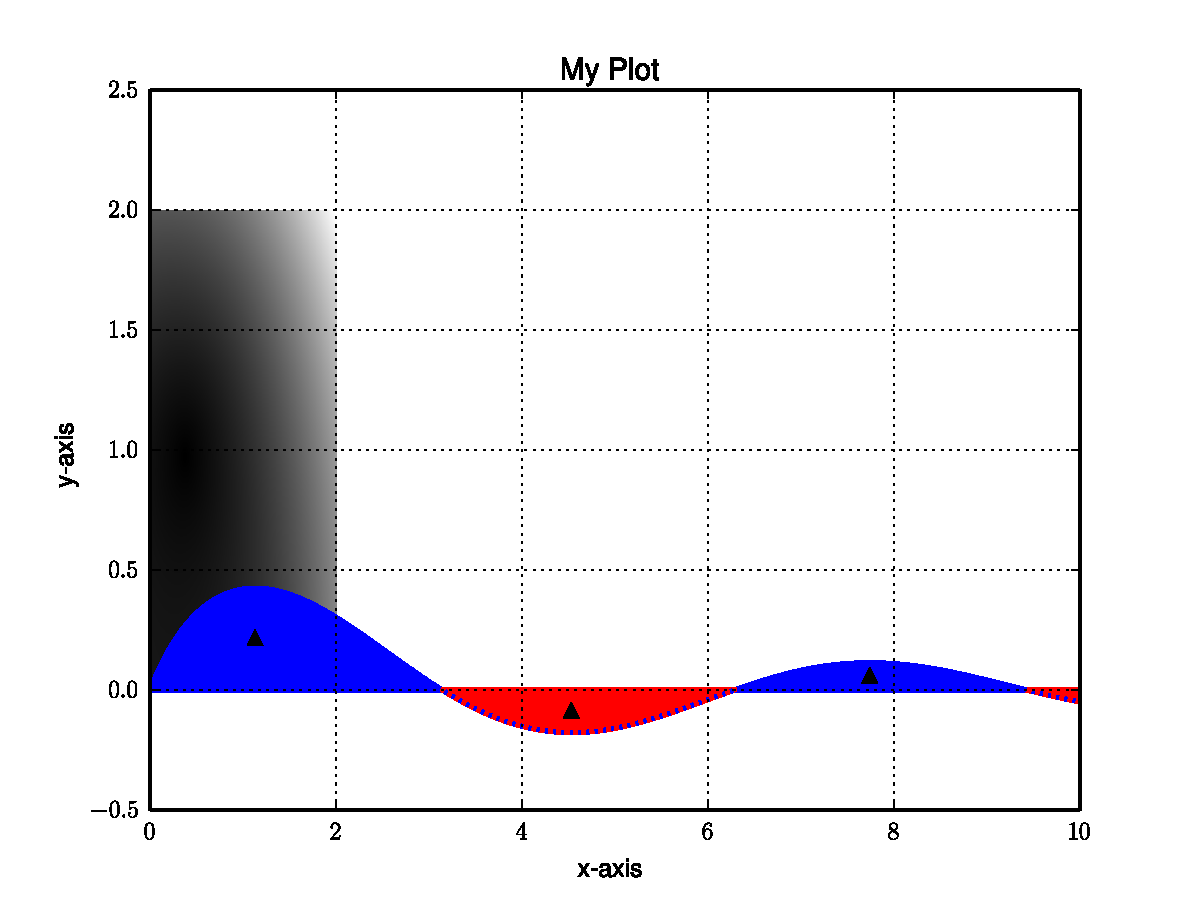
\includegraphics[width=\textwidth]{soln3.pdf}
\label{fig:problem3} 
\end{figure}
\end{problem}

\subsection*{pcolormesh}
Pcolormesh is a function in pyplot which produces a pseudocolor plot of a 2D array. 

The following is an example of using the pcolormesh function to represent 
the surface $z=\sin(x)\sin(y)$:
\begin{lstlisting}
n = 401 
x = np.linspace(-6, 6, n) 
y = np.linspace(-6, 6, n) 
X, Y = np.meshgrid(x, y) # returns a coordinate matrix given coordinate vectors. 
C = np.sin(X) * np.sin(Y) 
plt.pcolormesh(X, Y, C)
plt.show()
\end{lstlisting}
This plot is shown in Figure \ref{fig:pcmexample}
\begin{figure} 
\includegraphics[width=\textwidth]{pcolor.png}
\caption{Color plot of $\sin\left(x\right)\times\sin\left(y\right)$.}
\label{fig:pcmexample} 
\end{figure}

\begin{problem} Use plt.pcolormesh to plot the absolute value of the function $x^3 +2x^2 -x +3$ on the complex plane with 0 $\leq$ \li{x} $\leq$ 2 and 0 $\leq$ \li{y} $\leq$ 2. 

Your plot should look like the figure below.



\begin{figure}[H]
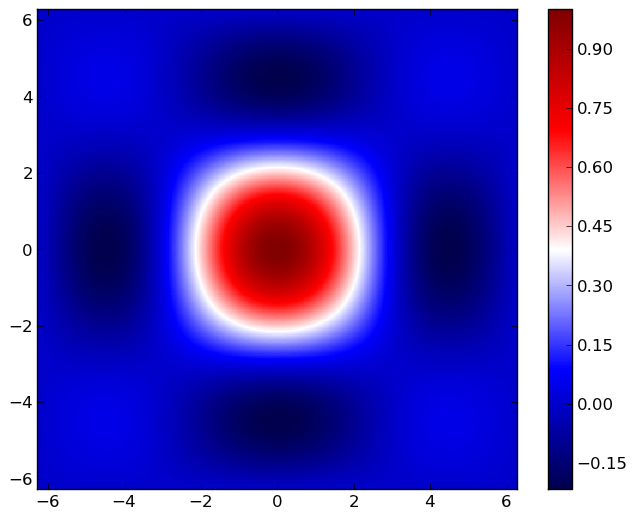
\includegraphics[width=\textwidth]{pcolor2.png}
\caption{Another example of a colorplot.} 
\label{fig:pcolormesh}
\end{figure}
\end{problem}

\begin{comment}

Matplotlib can also be used for 3D plotting. The following is an example
of how to use matplotlib to plot the function $z=\sin(x)\sin(y)$ with
both x and y ranging from -6 to 6. The resulting plot is shown in Figure
\ref{mpl:3dplot}. If you change the number of sample points used you
will notice that graphs look much nicer with large numbers of sample
points, but it will also take much longer for your computer to render
the image.

\begin{lstlisting} from mpl_toolkits.mplot3d import Axes3D from
matplotlib import pyplot as plt import numpy as np fig = plt.figure() ax
= fig.gca(projection='3d') x = np.linspace(-6, 6, 301) y =
np.linspace(-6, 6, 301) X, Y = np.meshgrid(x, y) Z = np.sin(X) *
np.sin(Y) ax.plot_surface(X, Y, Z) plt.show() \end{lstlisting}

\begin{figure} 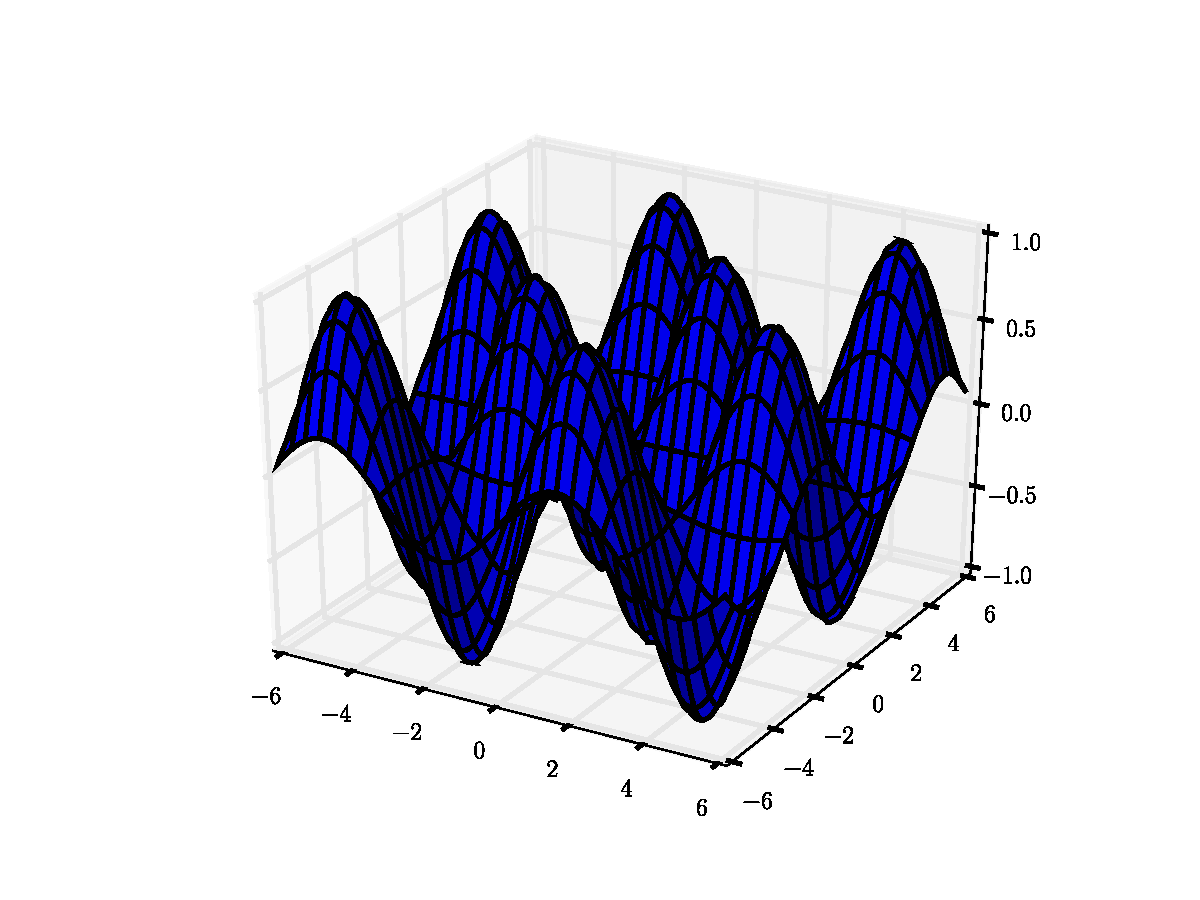
\includegraphics[width=\textwidth]{3dplot.pdf} \caption{A
3D plot of $\sin\left(x\right)\times\sin\left(y\right)$.}
\label{mpl:3dplot} \end{figure}

\begin{problem} Plot the function \begin{equation*}
\frac{\cos\left(\sqrt{x^2 + y^2}\right)}{\frac{x^2 + y^2}{10} + 1}
\end{equation*} on $[-10, 10] \times [-10, 10]$. \end{problem}


Matplotlib also allows us to make interactive graphs as follows:

% This example is largely based on one of the examples in the matplotlib
% docs. I have simplified it and changed the way the libraries are
% imported, but we could do a citation anyway.
% 
\begin{lstlisting} import numpy as np from matplotlib import pyplot as
plt from matplotlib import widgets as wg ax = plt.subplot(111)
plt.subplots_adjust(bottom=.25) t = np.arange(0., 1., .001) a0 = 5. f0 =
3. s = a0 * np.sin(2 * np.pi * f0 * t) l = plt.plot(t, s)[0]
plt.axis([0, 1, -10, 10]) axfreq = plt.axes([.25, .05, .65, .03]) axamp 
= plt.axes([.25, .1, .65, .03]) sfreq = wg.Slider(axfreq, 'Freq', .1,
30., valinit=f0) samp = wg.Slider(axamp, 'Amp', .1, 10., valinit=a0) def
update(val): amp = samp.val freq = sfreq.val l.set_ydata(amp * np.sin(2
* np.pi * freq * t)) plt.draw() sfreq.on_changed(update)
samp.on_changed(update) plt.show() \end{lstlisting} The resulting plot
is shown in Figure \ref{mpl:interact}.

\begin{figure} 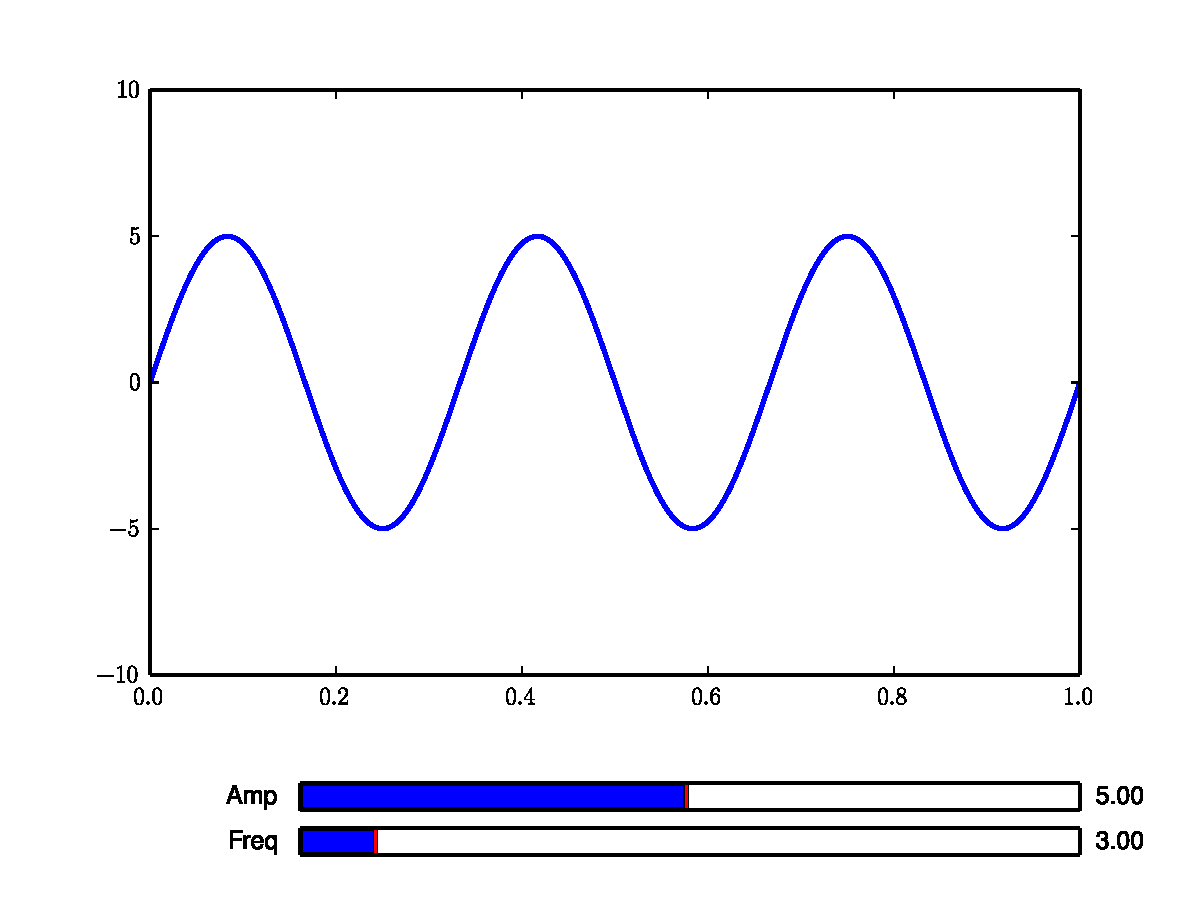
\includegraphics[width=\textwidth]{interact.pdf}
\caption{A snapshot of an interactive plot made using Matplotlib.}
\label{mpl:interact} \end{figure}

\begin{problem} Modify the code above to add a third slider to
manipulate the phase of the wave shown. Have it range from 0 to $2\pi$
and set the default value to zero. \end{problem}

\end{comment}

\section*{subplots}

We can plot multiple images at the same time using the \li{plt.subplot} command. 
It takes 3 arguments: the number of rows, the numer of columns, and the plot number. 
The plot number starts at 1 and increments first across the rows. 
For each subplot, preface the code needed with
\begin{lstlisting}
plt.subplot(nrows, ncols, plot_number)
\end{lstlisting}
However, if all the arguments are each less than 10, the commas can be 
omitted. 
\begin{lstlisting}
plt.subplot(nrowsncolsplot_number)
\end{lstlisting}
Note that with each subplot, only the plot number changes. 

The following example showcases plots of $sin x$ and $cos x$ on two 
different axes within the same plot.

Figure \ref{fig:subplots} is the output from the following code:
\begin{lstlisting}
x = np.linspace(-np.pi, np.pi, 400) 
y1 = np.sin(x) 
y2 = np.cos(x)
plt.subplot(211) 
plt.plot(x, y1) 
plt.subplot(212) 
plt.plot(x, y2)
plt.show() 
\end{lstlisting}

\begin{figure} 
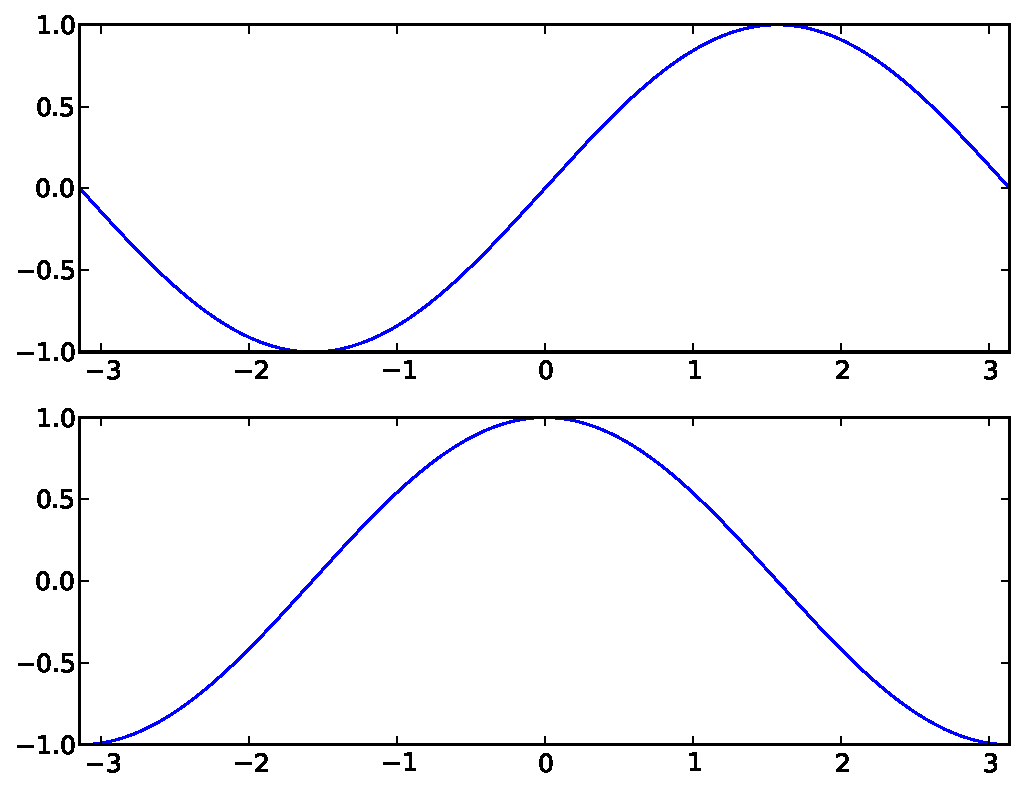
\includegraphics[width=\textwidth]{subplots.pdf}
\caption{An example of the use of subplots in Matplotlib.}
\label{fig:subplots} 
\end{figure}

\subsection*{Titles and Labels}

We can add titles to each subplot using the \li{plt.title} function. The
\li{plt.suptitle} function allows us to give the entire figure a title
as well.

\begin{problem} 
Make a plot with 4 subplots. In the subplots place graphs of $e^x$,
$sin(x)$, $cos(x)$, and $x^2$. Plot all of them on the interval
$(-\pi,\pi)$. Title each of them accordingly. Title the entire figure
``My Different Plots." 
\end{problem}

\begin{comment} 
%Table \ref{mpl:basics} 
\begin{table} 
\begin{center}
\begin{tabular}{|l|p{7cm}|p{3cm}|}

    \hline

    Function & Description & Usage\\

    \hline

    \li{bar} & makes a bar graph & bar(left,height)\\

    \li{barh} & makes a horizontal bar graph & barh(bottom,width)\\

    \li{fill} & plots lines with shading under the curve & fill(x,y)\\

    \li{fill\_between} & plots lines with shading between two given y
    values & fill\_ between(x,y1, y2=0)\\

    \li{hist} & plots a histogram from data & hist(data)\\

    \li{pie} & make a pie chart & pie(x)\\

    \li{plot} & plots lines and data on standard axes & plot(x,y)\\

    \li{polar} & plots lines and data on polar axes & polar(theta,r)\\

    \li{loglog} & plots lines and data on logarithmic x and y axes &
    loglog(x,y)\\

    \li{scatter} & plots data, has more options for scatter plots than
    the plot function & scatter(x,y)\\

    \li{semilogx} & plots lines and data with a log scaled x axis &
    semilogx(x,y)\\

    \li{semilogy} & plots lines and data with a log scaled y axis &
    semilogy(x,y)\\

    \li{specgram} & make a spectogram from data & specgram(x)\\

    \li{spy} & plot the sparsity pattern of a 2D array & spy(Z)\\

    \li{triplot} & plot triangulation between given points &
    triplot(x,y)\\

    \hline

    \end{tabular} 
    \end{center} 
    \caption{Some basic functions in Matplotlib.} 
    \label{mpl:basics} 
    \end{table} 
    
    
    \end{comment}

\section*{mayavi}
Matplotlib is the preferred library for 2D plotting. We will now
consider Mayavi for 3D plotting. It is a general scientific data
visualizer that seeks to provide interactive visualization of 3D data.
It provides easy integration with Python scientific libraries and
maintains a rich user interface that allows interaction with all data
and objects.

We encourage you to visit the formal documentation at
\url{docs.enthought.com/mayavi/mayavi/} for more information. 

In mayavi we will be using the \li{mlab} API which is imported like so
\begin{lstlisting}
from mayavi import mlab
\end{lstlisting}

\li{mlab} has many plotting functions including
\begin{itemize}
\item barchart
\item contour3d
\item flow
\item imshow
\item mesh
\item molecule
\item plot3d
\item points3d
\item quiver 3d
\item surf
\end{itemize}

All these can be "tested" by typing the command
\begin{lstlisting}
mlab.test_<plotting function>()
\end{lstlisting}
Note that pressing tab after typing \li{mlab.test_} will provide a 
list of available commands. 

To test the fancy mesh, type the following command
\begin{lstlisting}
mlab.test_fancy_mesh()
\end{lstlisting}

The result should resemble Figure \ref{fig:fancymesh}

\begin{figure} 
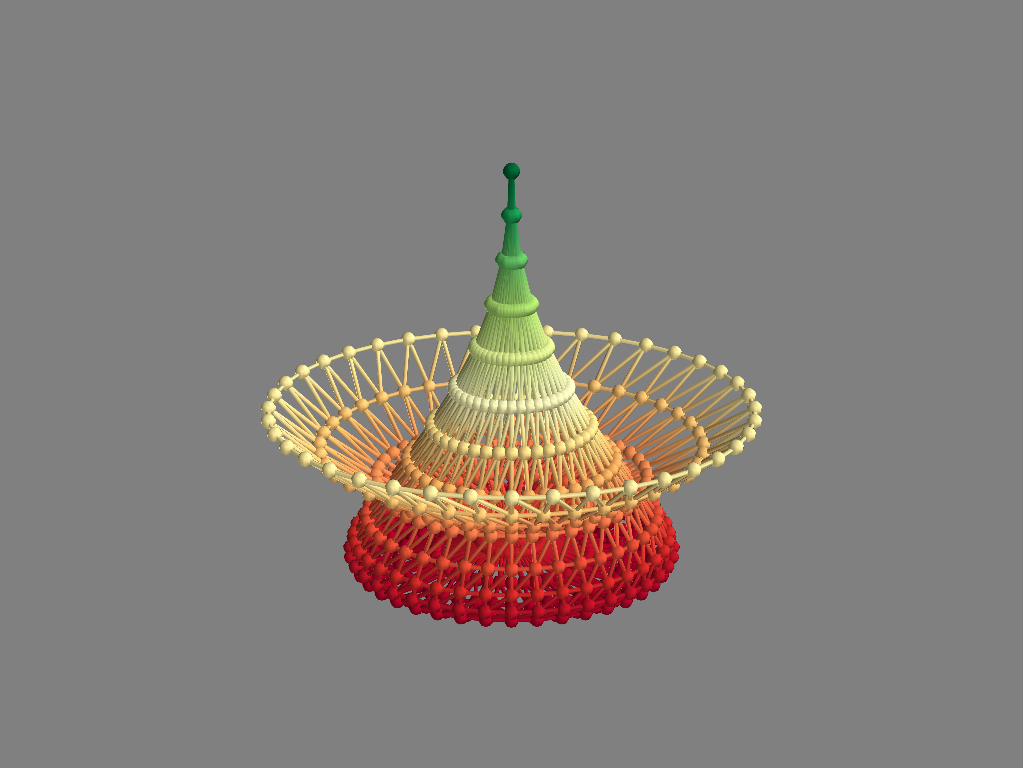
\includegraphics[width=\textwidth]{fancymesh.png}
\caption{An example of the fancy mesh plotting function} 
\label{fig:fancymesh}
\end{figure}


We will focus our attention on introducing the \li{surf}, \li{mesh}, 
\li{plot3d}, and \li{points3d} functions. 


\subsection*{3D Plotting} Similar to matplotlib, \li{mlab} takes a set
of data points and plots it. Instead of passing just \li{x} and \li{y}
coordinates like we did in matplotlib, we will also send \li{z}
coordinates to produce a 3D plot. 

\subsection*{surf}
The \li{surf} function is great for simple structures like orthogonal grids 
because it will create efficient data structures. 
It is common to use 2D arrays returned by \li{np.meshgrid}. 

For more complex structures, the \li{mesh} function is more appropriate. 

\subsection*{mesh}
\li{mesh} plots a surface using grid-spaced data. 
It expects three 2D numpy arrays. As with matplotlib, it is important that 
all three arrays to be the same shape. 

\subsection*{plot3d}
\li{plot3d} is used to draw lines between points. It expects three numpy 
arrays to provide the position of the line. 

The following illustrates a simple floral design.
\begin{lstlisting}
from mayavi import mlab

num = np.pi/1000
pts = np.arange(0, 2*np.pi + num, num)
x = np.cos(pts) * (1 + np.cos(pts*6))
y = np.sin(pts) * (1 + np.cos(pts*6))
z = np.sin(pts*6/11)
mlab.plot3d(x, y, z)
\end{lstlisting}
This will produce Figure \ref{fig:plot3d}
\begin{figure} 

\includegraphics[width=\textwidth]{plot3d.png}
\caption{A simple floral.} 
\label{fig:plot3d}
\end{figure}


\subsection*{points3d}
\li{points3d} is very similar to \li{plot3d} except it plots glyphs at the 
position of the supplied data. It takes the same arguments. This time we 
will use a keyword argument, \li{s}, which provides an associated scalar 
value for each point given. It modifies the size and color of the points. 

The following illustrates a simple heart - given the right perspective. 
\begin{lstlisting}
pts = np.linspace(0, 4 * np.pi, 30)
x = np.sin(2 * pts)
y = np.cos(pts)
z = np.cos(2 * pts)
s = 2+np.sin(pts)
mlab.points3d(x, y, z, s, colormap="cool", scale_factor=.15)
mlab.savefig("testpoints3d.png", size=(1024,768))
\end{lstlisting}
This will produce Figure \ref{fig:points3d}

\begin{figure} 
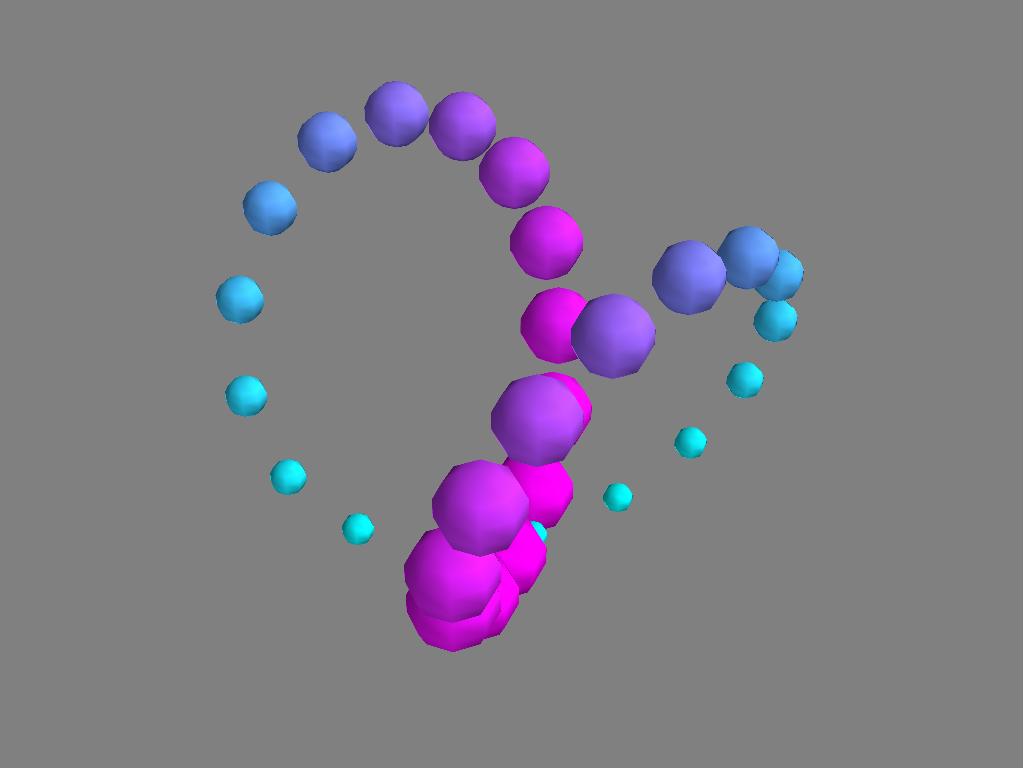
\includegraphics[width=\textwidth]{points3d.png}
\caption{A simple heart.} 
\label{fig:points3d}
\end{figure}

\subsection*{Changing Looks}
The color of your object can be explicitly defined using the \li{color} 
keyword argument. It is specified as a triplet (red, green, blue) of 
floating points ranging from 0 to 1. 
For example, (1.0, 1.0, 1.0) is white. 

If, however, you would prefer to vary the colors across your visualization, 
using a colormap is suggested. Table \ref{table:colormaps} provides 
all possible colormaps. 

\begin{table} 
\begin{center}
\begin{tabular}{|l|c|r|}
\hline
\multicolumn{2}{c}
{Colormaps} \\
\hline
\li{Accent} & \li{autumn} & \li{black-white} \\
\li{blue-red} & \li{Blues} & \li{bone} \\
\li{BrBG} & \li{BuGn} & \li{BuPu} \\
\li{cool} & \li{copper} & \li{Dark2} \\
\li{flag} & \li{gist_earth} & \li{gist_gray} \\
\li{gist_heat} & \li{gist_ncar} & \li{gist_rainbow} \\
\li{gist_stern} & \li{gist_yarg} & \li{GnBu} \\
\li{gray} & \li{Greens} & \li{Greys} \\
\li{hot} & \li{hsv} & \li{jet} \\
\li{Oranges} & \li{OrRd} & \li{Paired} \\
\li{Pastel1} & \li{Pastel2} & \li{pink} \\
\li{PiYG} & \li{PRGn} & \li{prism} \\
\li{PuBu} & \li{PuBuGn} & \li{PuOr} \\
\li{PuRd} & \li{PurpLes} & \li{RdBu} \\
\li{RdGy} & \li{RdPu} & \li{RdYlBu} \\
\li{RdYlGn} & \li{Reds} & \li{Setl} \\
\li{Set2} & \li{Set3} & \li{Spectral} \\
\li{spring} & \li{summer} & \li{winter} \\
\li{YlGnBu} & \li{YlGn} & \li{YlOrRd} \\
\li{YlOrBr} \\
\hline
\end{tabular} 
\end{center} 
\caption{Colormaps} 
\label{table:colormaps} 
\end{table} 


\subsection*{Useful Features} 
One of the most useful features in \li{mayavi} is the record feature. 
In the pipeline view (far left corner) there is a round, red button. 
Clicking it opens a recorder that keeps track of all the changes made 
interactively to the visualization. It also generates valid lines of Python code. 

\begin{problem} 
Provided Grand Canyon topological radar data from NASA, 
do the following.

\begin{itemize}
\item resize the data to be 3601x3601
\item Cast the type of be \li{float32}. 
\item Resize the data to take the first 1000 rows and columns 900-1900.
\item There is some missing data so set the minimum of your data equal to the minimum of the the positive data points. 
\item Do the following to preset the figure. mlab.figure(size=(400,320), bgcolor = (.16, .28, .46))
\item Now plot using mlab.surf using the colormap gist earth with a warp scale of .2, vmin of 1200, and a vmax of 1610.
\item Take a smaller view of the canyon. mlab.view(-5.9, 83, 570, [5.3, 20, 238])
\end{itemize}

This should result in Figure \ref{fig:GrandCanyon}
\end{problem}

\begin{figure} 
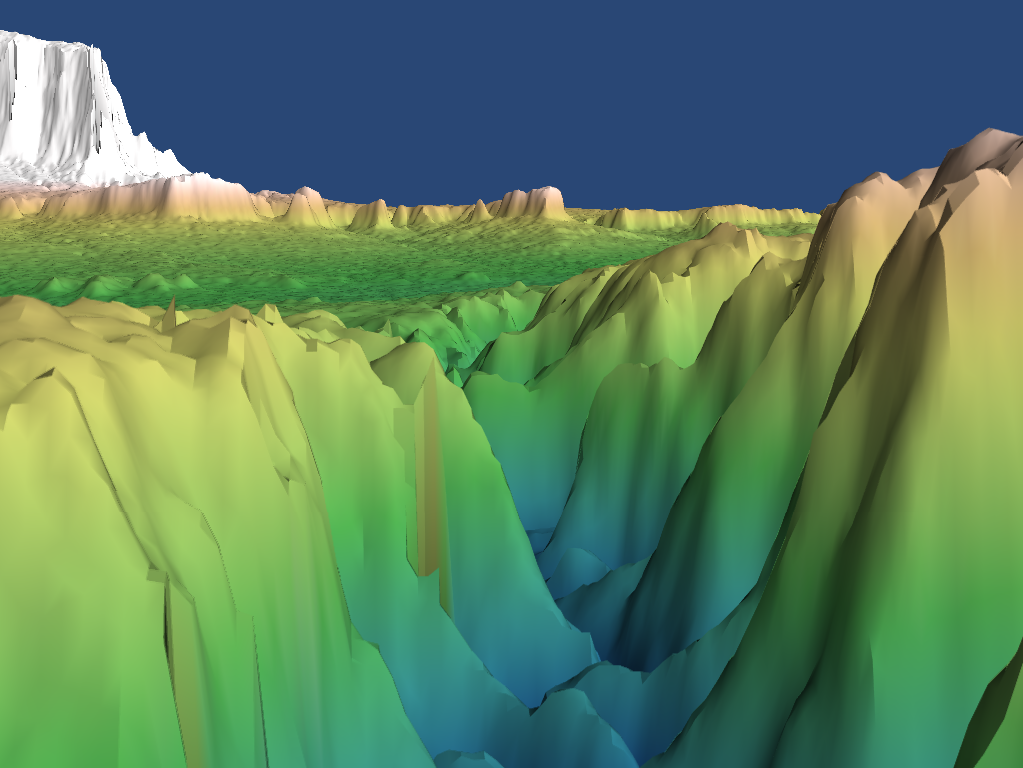
\includegraphics[width=\textwidth]{GrandCanyon.png}
\caption{A view of the Grand Canyon} 
\label{fig:GrandCanyon}
\end{figure}

